\documentclass{beamer}

\title{Raven Comparison Statistics}
\author{Josh Cogliati\\ (and this would not have happened without\\ Ivan Rinaldi and Cristian Rabiti)}


\begin{document}

\begin{frame}
  \titlepage
\end{frame}

\begin{frame}
  \frametitle{Outline}
  \tableofcontents
\end{frame}

\section{Motivation}

\begin{frame}
  \frametitle{Why are we doing this?}
  We have codes that we need to compare to each other and to experiments.
\end{frame}

\begin{frame}
  \frametitle{Example}
  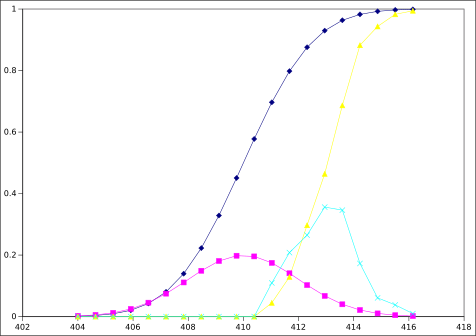
\includegraphics[height=6cm]{example}
\end{frame}

\section{Comparisons}

%cdf area difference
\begin{frame}
  \frametitle{CDF difference area}
  This calculates the difference in area between the two CDFs
  \begin{equation}
    cdf\_area\_difference = \int_{-\infty}^{\infty}{\|CDF_a(x)-CDF_b(x)\|dx}
  \end{equation}
  \begin{columns}
    \column{.5\textwidth}
    \includegraphics[height=3cm]{example_cdf_area}
    \column{.5\textwidth}
    Note that this area will have the same units as x.
  \end{columns}
\end{frame}

%common pdf area
\begin{frame}
  \frametitle{Common PDF area}
  This calculates the common area between the two PDFs.
  \begin{equation}
    pdf\_common\_area = \int_{-\infty}^{\infty}{\min(PDF_a(x),PDF_b(x))}dx
  \end{equation}
  \begin{columns}
    \column{.5\textwidth}
    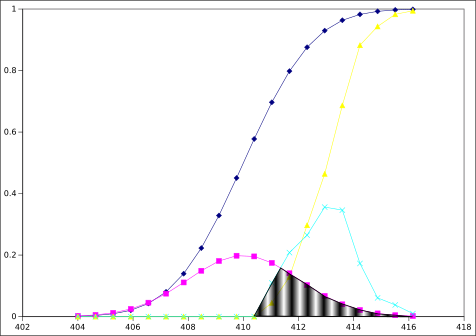
\includegraphics[height=3cm]{example_pdf_common}
    \column{.5\textwidth}
    This will range from 0\% to 100\%, with 100\% being a complete match.
  \end{columns}
\end{frame}


%difference between pdfs
\begin{frame}
  \frametitle{Difference between PDFs}
  This calculates a difference between the PDFs.
  \begin{equation}
    f_Z(z) = \int_{-\infty}^{\infty}f_X(x)f_Y(x-z)dx
  \end{equation}
  \begin{columns}
    \column{0.5\textwidth}
    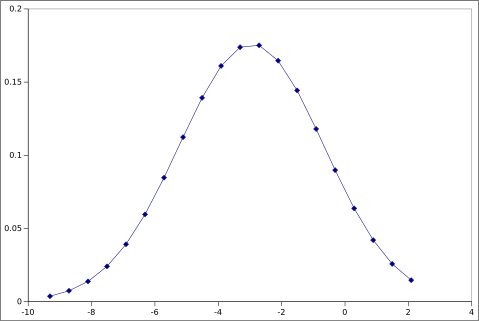
\includegraphics[height=3cm]{f_z}
    \column{0.5\textwidth}
    This generates a new pdf, with mean related
    to the average difference, and variance depending on a variety of
    factors.
  \end{columns}
\end{frame}

\begin{frame}
  \frametitle{Use of Differences between PDFs}
  This calculates the average:
  \begin{equation}
    \bar{z} = \int_{-\infty}^{\infty}{z f_Z(z)dz}
  \end{equation}
  This calculates the variance:
  \begin{equation}
    var = \int_{-\infty}^{\infty}{(z-\bar{z})^2 f_Z(z)dz}
  \end{equation}
\end{frame}

\section{Implementation}

%getting bins

%creating interpolation functions

%integrating

\section{Future Directions}



\end{document}
